% Created by tikzDevice version 0.12.6 on 2025-02-12 13:10:24
% !TEX encoding = UTF-8 Unicode
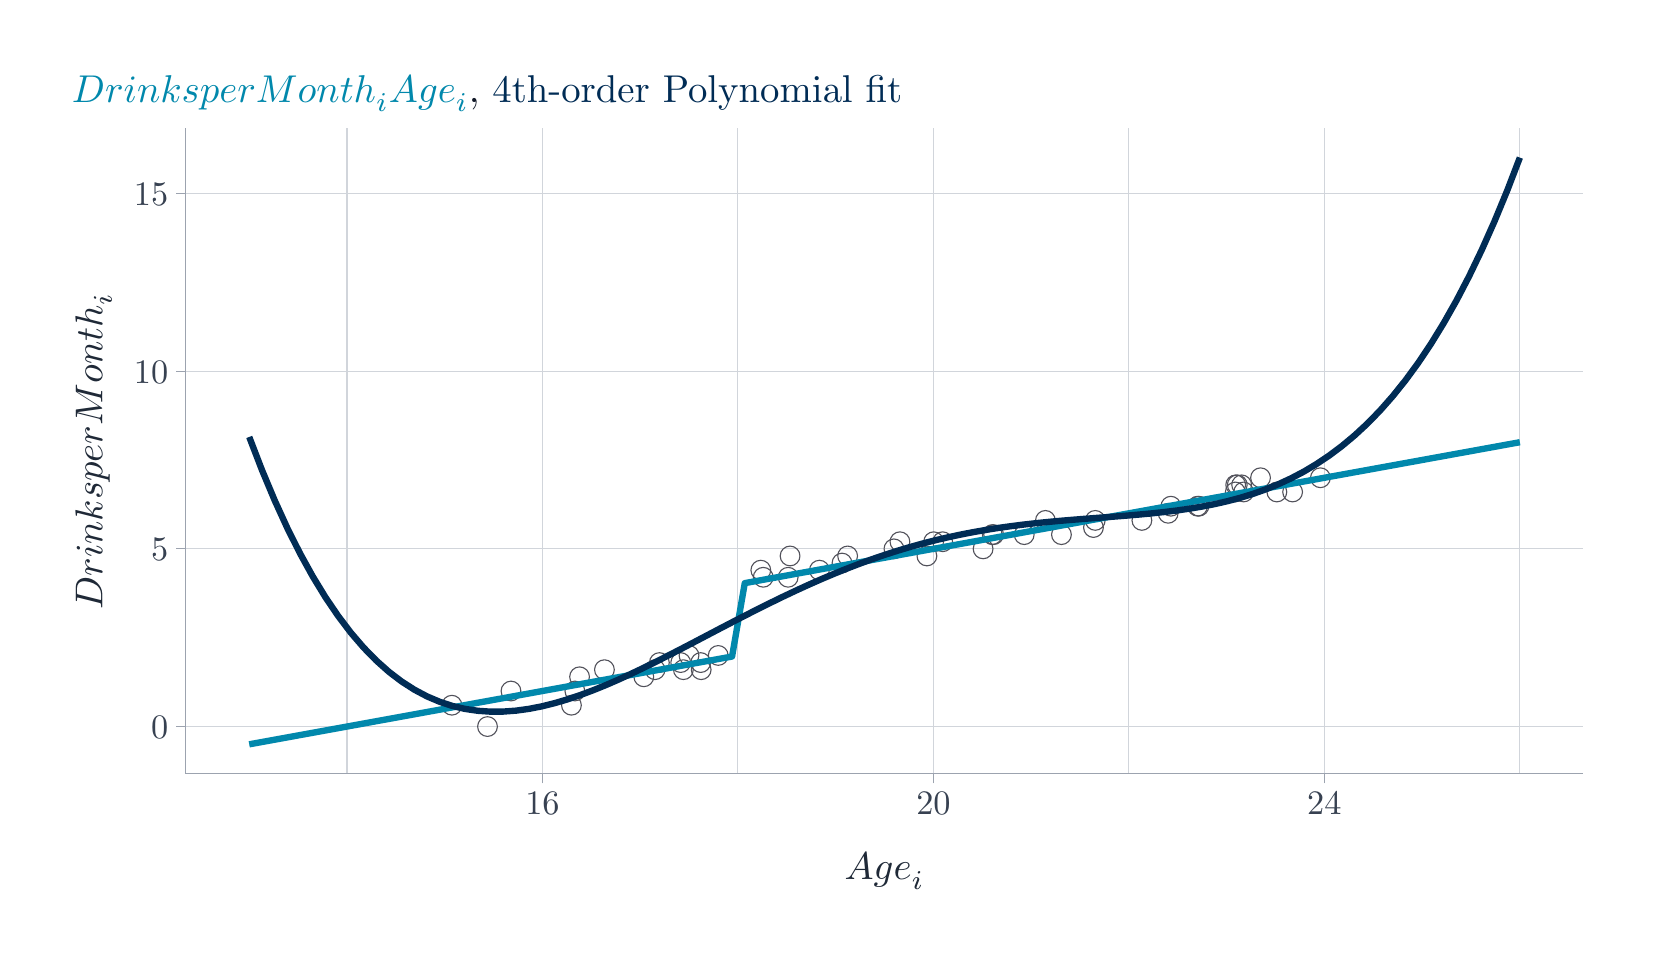
\begin{tikzpicture}[x=1pt,y=1pt]
\definecolor{fillColor}{RGB}{255,255,255}
\path[use as bounding box,fill=fillColor] (0,0) rectangle (578.16,325.21);
\begin{scope}
\path[clip] (  0.00,  0.00) rectangle (578.16,325.21);
\definecolor{drawColor}{RGB}{255,255,255}

\path[draw=drawColor,line width= 0.7pt,line join=round,line cap=round,fill=fillColor] (  0.00,  0.00) rectangle (578.16,325.21);
\end{scope}
\begin{scope}
\path[clip] ( 57.10, 55.65) rectangle (562.16,288.85);
\definecolor{drawColor}{RGB}{255,255,255}
\definecolor{fillColor}{RGB}{255,255,255}

\path[draw=drawColor,line width= 0.7pt,line join=round,line cap=round,fill=fillColor] ( 57.10, 55.65) rectangle (562.16,288.85);
\definecolor{drawColor}{RGB}{209,213,219}

\path[draw=drawColor,line width= 0.4pt,line join=round] (115.38, 55.65) --
	(115.38,288.85);

\path[draw=drawColor,line width= 0.4pt,line join=round] (256.65, 55.65) --
	(256.65,288.85);

\path[draw=drawColor,line width= 0.4pt,line join=round] (397.93, 55.65) --
	(397.93,288.85);

\path[draw=drawColor,line width= 0.4pt,line join=round] (539.20, 55.65) --
	(539.20,288.85);

\path[draw=drawColor,line width= 0.4pt,line join=round] ( 57.10, 72.67) --
	(562.16, 72.67);

\path[draw=drawColor,line width= 0.4pt,line join=round] ( 57.10,136.88) --
	(562.16,136.88);

\path[draw=drawColor,line width= 0.4pt,line join=round] ( 57.10,201.10) --
	(562.16,201.10);

\path[draw=drawColor,line width= 0.4pt,line join=round] ( 57.10,265.31) --
	(562.16,265.31);

\path[draw=drawColor,line width= 0.4pt,line join=round] (186.01, 55.65) --
	(186.01,288.85);

\path[draw=drawColor,line width= 0.4pt,line join=round] (327.29, 55.65) --
	(327.29,288.85);

\path[draw=drawColor,line width= 0.4pt,line join=round] (468.57, 55.65) --
	(468.57,288.85);
\definecolor{drawColor}{RGB}{82,82,91}

\path[draw=drawColor,line width= 0.4pt,line join=round,line cap=round] (243.20, 95.79) circle (  3.57);

\path[draw=drawColor,line width= 0.4pt,line join=round,line cap=round] (236.94, 93.22) circle (  3.57);

\path[draw=drawColor,line width= 0.4pt,line join=round,line cap=round] (174.64, 85.51) circle (  3.57);

\path[draw=drawColor,line width= 0.4pt,line join=round,line cap=round] (226.70, 93.22) circle (  3.57);

\path[draw=drawColor,line width= 0.4pt,line join=round,line cap=round] (166.16, 72.67) circle (  3.57);

\path[draw=drawColor,line width= 0.4pt,line join=round,line cap=round] (327.37,139.45) circle (  3.57);

\path[draw=drawColor,line width= 0.4pt,line join=round,line cap=round] (243.37, 93.22) circle (  3.57);

\path[draw=drawColor,line width= 0.4pt,line join=round,line cap=round] (265.79,126.61) circle (  3.57);

\path[draw=drawColor,line width= 0.4pt,line join=round,line cap=round] (348.56,142.02) circle (  3.57);

\path[draw=drawColor,line width= 0.4pt,line join=round,line cap=round] (296.29,134.31) circle (  3.57);

\path[draw=drawColor,line width= 0.4pt,line join=round,line cap=round] (437.08,160.00) circle (  3.57);

\path[draw=drawColor,line width= 0.4pt,line join=round,line cap=round] (413.09,152.29) circle (  3.57);

\path[draw=drawColor,line width= 0.4pt,line join=round,line cap=round] (264.92,129.18) circle (  3.57);

\path[draw=drawColor,line width= 0.4pt,line join=round,line cap=round] (402.62,147.16) circle (  3.57);

\path[draw=drawColor,line width= 0.4pt,line join=round,line cap=round] (196.49, 80.38) circle (  3.57);

\path[draw=drawColor,line width= 0.4pt,line join=round,line cap=round] (249.53, 98.36) circle (  3.57);

\path[draw=drawColor,line width= 0.4pt,line join=round,line cap=round] (238.97, 98.36) circle (  3.57);

\path[draw=drawColor,line width= 0.4pt,line join=round,line cap=round] (197.73, 85.51) circle (  3.57);

\path[draw=drawColor,line width= 0.4pt,line join=round,line cap=round] (274.80,126.61) circle (  3.57);

\path[draw=drawColor,line width= 0.4pt,line join=round,line cap=round] (436.51,160.00) circle (  3.57);

\path[draw=drawColor,line width= 0.4pt,line join=round,line cap=round] (385.12,144.59) circle (  3.57);

\path[draw=drawColor,line width= 0.4pt,line join=round,line cap=round] (294.25,131.75) circle (  3.57);

\path[draw=drawColor,line width= 0.4pt,line join=round,line cap=round] (275.49,134.31) circle (  3.57);

\path[draw=drawColor,line width= 0.4pt,line join=round,line cap=round] (412.12,149.73) circle (  3.57);

\path[draw=drawColor,line width= 0.4pt,line join=round,line cap=round] (439.38,157.43) circle (  3.57);

\path[draw=drawColor,line width= 0.4pt,line join=round,line cap=round] (313.02,136.88) circle (  3.57);

\path[draw=drawColor,line width= 0.4pt,line join=round,line cap=round] (208.41, 93.22) circle (  3.57);

\path[draw=drawColor,line width= 0.4pt,line join=round,line cap=round] (436.37,157.43) circle (  3.57);

\path[draw=drawColor,line width= 0.4pt,line join=round,line cap=round] (286.09,129.18) circle (  3.57);

\path[draw=drawColor,line width= 0.4pt,line join=round,line cap=round] (438.67,160.00) circle (  3.57);

\path[draw=drawColor,line width= 0.4pt,line join=round,line cap=round] (467.13,162.57) circle (  3.57);

\path[draw=drawColor,line width= 0.4pt,line join=round,line cap=round] (451.39,157.43) circle (  3.57);

\path[draw=drawColor,line width= 0.4pt,line join=round,line cap=round] (349.05,142.02) circle (  3.57);

\path[draw=drawColor,line width= 0.4pt,line join=round,line cap=round] (385.76,147.16) circle (  3.57);

\path[draw=drawColor,line width= 0.4pt,line join=round,line cap=round] (422.73,152.29) circle (  3.57);

\path[draw=drawColor,line width= 0.4pt,line join=round,line cap=round] (360.10,142.02) circle (  3.57);

\path[draw=drawColor,line width= 0.4pt,line join=round,line cap=round] (235.97, 95.79) circle (  3.57);

\path[draw=drawColor,line width= 0.4pt,line join=round,line cap=round] (330.64,139.45) circle (  3.57);

\path[draw=drawColor,line width= 0.4pt,line join=round,line cap=round] (457.08,157.43) circle (  3.57);

\path[draw=drawColor,line width= 0.4pt,line join=round,line cap=round] (315.19,139.45) circle (  3.57);

\path[draw=drawColor,line width= 0.4pt,line join=round,line cap=round] (228.27, 95.79) circle (  3.57);

\path[draw=drawColor,line width= 0.4pt,line join=round,line cap=round] (445.49,162.57) circle (  3.57);

\path[draw=drawColor,line width= 0.4pt,line join=round,line cap=round] (345.24,136.88) circle (  3.57);

\path[draw=drawColor,line width= 0.4pt,line join=round,line cap=round] (423.23,152.29) circle (  3.57);

\path[draw=drawColor,line width= 0.4pt,line join=round,line cap=round] (222.64, 90.65) circle (  3.57);

\path[draw=drawColor,line width= 0.4pt,line join=round,line cap=round] (199.42, 90.65) circle (  3.57);

\path[draw=drawColor,line width= 0.4pt,line join=round,line cap=round] (367.76,147.16) circle (  3.57);

\path[draw=drawColor,line width= 0.4pt,line join=round,line cap=round] (373.55,142.02) circle (  3.57);

\path[draw=drawColor,line width= 0.4pt,line join=round,line cap=round] (153.29, 80.38) circle (  3.57);

\path[draw=drawColor,line width= 0.4pt,line join=round,line cap=round] (324.94,134.31) circle (  3.57);
\definecolor{drawColor}{RGB}{1,136,172}

\path[draw=drawColor,line width= 2.3pt,line join=round] ( 80.06, 66.25) --
	( 84.65, 67.08) --
	( 89.24, 67.92) --
	( 93.83, 68.75) --
	( 98.42, 69.59) --
	(103.02, 70.42) --
	(107.61, 71.26) --
	(112.20, 72.09) --
	(116.79, 72.93) --
	(121.38, 73.76) --
	(125.97, 74.60) --
	(130.56, 75.43) --
	(135.16, 76.27) --
	(139.75, 77.10) --
	(144.34, 77.94) --
	(148.93, 78.77) --
	(153.52, 79.61) --
	(158.11, 80.44) --
	(162.70, 81.28) --
	(167.30, 82.11) --
	(171.89, 82.94) --
	(176.48, 83.78) --
	(181.07, 84.61) --
	(185.66, 85.45) --
	(190.25, 86.28) --
	(194.84, 87.12) --
	(199.44, 87.95) --
	(204.03, 88.79) --
	(208.62, 89.62) --
	(213.21, 90.46) --
	(217.80, 91.29) --
	(222.39, 92.13) --
	(226.98, 92.96) --
	(231.58, 93.80) --
	(236.17, 94.63) --
	(240.76, 95.47) --
	(245.35, 96.30) --
	(249.94, 97.14) --
	(254.53, 97.97) --
	(259.12,124.49) --
	(263.72,125.33) --
	(268.31,126.16) --
	(272.90,126.99) --
	(277.49,127.83) --
	(282.08,128.66) --
	(286.67,129.50) --
	(291.26,130.33) --
	(295.86,131.17) --
	(300.45,132.00) --
	(305.04,132.84) --
	(309.63,133.67) --
	(314.22,134.51) --
	(318.81,135.34) --
	(323.40,136.18) --
	(328.00,137.01) --
	(332.59,137.85) --
	(337.18,138.68) --
	(341.77,139.52) --
	(346.36,140.35) --
	(350.95,141.19) --
	(355.54,142.02) --
	(360.14,142.86) --
	(364.73,143.69) --
	(369.32,144.52) --
	(373.91,145.36) --
	(378.50,146.19) --
	(383.09,147.03) --
	(387.68,147.86) --
	(392.28,148.70) --
	(396.87,149.53) --
	(401.46,150.37) --
	(406.05,151.20) --
	(410.64,152.04) --
	(415.23,152.87) --
	(419.83,153.71) --
	(424.42,154.54) --
	(429.01,155.38) --
	(433.60,156.21) --
	(438.19,157.05) --
	(442.78,157.88) --
	(447.37,158.72) --
	(451.97,159.55) --
	(456.56,160.39) --
	(461.15,161.22) --
	(465.74,162.05) --
	(470.33,162.89) --
	(474.92,163.72) --
	(479.51,164.56) --
	(484.11,165.39) --
	(488.70,166.23) --
	(493.29,167.06) --
	(497.88,167.90) --
	(502.47,168.73) --
	(507.06,169.57) --
	(511.65,170.40) --
	(516.25,171.24) --
	(520.84,172.07) --
	(525.43,172.91) --
	(530.02,173.74) --
	(534.61,174.58) --
	(539.20,175.41);
\definecolor{drawColor}{RGB}{0,44,85}

\path[draw=drawColor,line width= 2.3pt,line join=round] ( 80.06,177.31) --
	( 84.65,165.39) --
	( 89.24,154.43) --
	( 93.83,144.38) --
	( 98.42,135.22) --
	(103.02,126.90) --
	(107.61,119.37) --
	(112.20,112.61) --
	(116.79,106.57) --
	(121.38,101.22) --
	(125.97, 96.52) --
	(130.56, 92.43) --
	(135.16, 88.93) --
	(139.75, 85.98) --
	(144.34, 83.55) --
	(148.93, 81.60) --
	(153.52, 80.10) --
	(158.11, 79.03) --
	(162.70, 78.36) --
	(167.30, 78.05) --
	(171.89, 78.08) --
	(176.48, 78.42) --
	(181.07, 79.05) --
	(185.66, 79.94) --
	(190.25, 81.08) --
	(194.84, 82.42) --
	(199.44, 83.96) --
	(204.03, 85.67) --
	(208.62, 87.52) --
	(213.21, 89.51) --
	(217.80, 91.61) --
	(222.39, 93.80) --
	(226.98, 96.06) --
	(231.58, 98.39) --
	(236.17,100.75) --
	(240.76,103.14) --
	(245.35,105.55) --
	(249.94,107.96) --
	(254.53,110.35) --
	(259.12,112.72) --
	(263.72,115.05) --
	(268.31,117.34) --
	(272.90,119.58) --
	(277.49,121.75) --
	(282.08,123.85) --
	(286.67,125.88) --
	(291.26,127.82) --
	(295.86,129.68) --
	(300.45,131.45) --
	(305.04,133.12) --
	(309.63,134.69) --
	(314.22,136.16) --
	(318.81,137.54) --
	(323.40,138.81) --
	(328.00,139.99) --
	(332.59,141.06) --
	(337.18,142.05) --
	(341.77,142.94) --
	(346.36,143.74) --
	(350.95,144.47) --
	(355.54,145.11) --
	(360.14,145.69) --
	(364.73,146.20) --
	(369.32,146.66) --
	(373.91,147.08) --
	(378.50,147.46) --
	(383.09,147.82) --
	(387.68,148.17) --
	(392.28,148.51) --
	(396.87,148.87) --
	(401.46,149.26) --
	(406.05,149.69) --
	(410.64,150.18) --
	(415.23,150.74) --
	(419.83,151.40) --
	(424.42,152.17) --
	(429.01,153.07) --
	(433.60,154.12) --
	(438.19,155.34) --
	(442.78,156.75) --
	(447.37,158.38) --
	(451.97,160.25) --
	(456.56,162.38) --
	(461.15,164.80) --
	(465.74,167.54) --
	(470.33,170.61) --
	(474.92,174.05) --
	(479.51,177.89) --
	(484.11,182.15) --
	(488.70,186.87) --
	(493.29,192.08) --
	(497.88,197.80) --
	(502.47,204.07) --
	(507.06,210.93) --
	(511.65,218.41) --
	(516.25,226.53) --
	(520.84,235.35) --
	(525.43,244.89) --
	(530.02,255.20) --
	(534.61,266.30) --
	(539.20,278.25);
\end{scope}
\begin{scope}
\path[clip] (  0.00,  0.00) rectangle (578.16,325.21);
\definecolor{drawColor}{RGB}{156,163,175}

\path[draw=drawColor,line width= 0.3pt,line join=round] ( 57.10, 55.65) --
	( 57.10,288.85);
\end{scope}
\begin{scope}
\path[clip] (  0.00,  0.00) rectangle (578.16,325.21);
\definecolor{drawColor}{RGB}{55,65,81}

\node[text=drawColor,anchor=base east,inner sep=0pt, outer sep=0pt, scale=  1.24] at ( 50.80, 68.39) {0};

\node[text=drawColor,anchor=base east,inner sep=0pt, outer sep=0pt, scale=  1.24] at ( 50.80,132.60) {5};

\node[text=drawColor,anchor=base east,inner sep=0pt, outer sep=0pt, scale=  1.24] at ( 50.80,196.81) {10};

\node[text=drawColor,anchor=base east,inner sep=0pt, outer sep=0pt, scale=  1.24] at ( 50.80,261.02) {15};
\end{scope}
\begin{scope}
\path[clip] (  0.00,  0.00) rectangle (578.16,325.21);
\definecolor{drawColor}{RGB}{156,163,175}

\path[draw=drawColor,line width= 0.3pt,line join=round] ( 53.60, 72.67) --
	( 57.10, 72.67);

\path[draw=drawColor,line width= 0.3pt,line join=round] ( 53.60,136.88) --
	( 57.10,136.88);

\path[draw=drawColor,line width= 0.3pt,line join=round] ( 53.60,201.10) --
	( 57.10,201.10);

\path[draw=drawColor,line width= 0.3pt,line join=round] ( 53.60,265.31) --
	( 57.10,265.31);
\end{scope}
\begin{scope}
\path[clip] (  0.00,  0.00) rectangle (578.16,325.21);
\definecolor{drawColor}{RGB}{156,163,175}

\path[draw=drawColor,line width= 0.3pt,line join=round] ( 57.10, 55.65) --
	(562.16, 55.65);
\end{scope}
\begin{scope}
\path[clip] (  0.00,  0.00) rectangle (578.16,325.21);
\definecolor{drawColor}{RGB}{156,163,175}

\path[draw=drawColor,line width= 0.3pt,line join=round] (186.01, 52.15) --
	(186.01, 55.65);

\path[draw=drawColor,line width= 0.3pt,line join=round] (327.29, 52.15) --
	(327.29, 55.65);

\path[draw=drawColor,line width= 0.3pt,line join=round] (468.57, 52.15) --
	(468.57, 55.65);
\end{scope}
\begin{scope}
\path[clip] (  0.00,  0.00) rectangle (578.16,325.21);
\definecolor{drawColor}{RGB}{55,65,81}

\node[text=drawColor,anchor=base,inner sep=0pt, outer sep=0pt, scale=  1.24] at (186.01, 40.78) {16};

\node[text=drawColor,anchor=base,inner sep=0pt, outer sep=0pt, scale=  1.24] at (327.29, 40.78) {20};

\node[text=drawColor,anchor=base,inner sep=0pt, outer sep=0pt, scale=  1.24] at (468.57, 40.78) {24};
\end{scope}
\begin{scope}
\path[clip] (  0.00,  0.00) rectangle (578.16,325.21);
\definecolor{drawColor}{RGB}{31,41,55}

\node[text=drawColor,anchor=base,inner sep=0pt, outer sep=0pt, scale=  1.40] at (309.63, 17.36) {$\text{Age}_i$};
\end{scope}
\begin{scope}
\path[clip] (  0.00,  0.00) rectangle (578.16,325.21);
\definecolor{drawColor}{RGB}{31,41,55}

\node[text=drawColor,rotate= 90.00,anchor=base,inner sep=0pt, outer sep=0pt, scale=  1.40] at ( 27.00,172.25) {$\text{Drinks per Month}_i$};
\end{scope}
\begin{scope}
\path[clip] (  0.00,  0.00) rectangle (578.16,325.21);
\definecolor{drawColor}{RGB}{17,24,39}

\node[text=drawColor,anchor=base west,inner sep=0pt, outer sep=0pt, scale=  1.40] at ( 16.00,298.21) {{\color[HTML]{0188AC} $\expec{\text{Drinks per Month}_i}{\text{Age}_i}$}, {\color[HTML]{002C55} 4th-order Polynomial fit}};
\end{scope}
\end{tikzpicture}
